	% Nama Kelompok : Kelompok 2
% Kelas : D4 TI 1A
% 1. Kadek Diva Krishna Murti (1174006)
% 2. Duvan Silalahi (1174011)
% 3. Oniwaldus (1174005)
% 4. Choirul Anam (1174004)
% 5. Sri Rahayu (1174015)
% 6. Ilham Habibi (1174028)

\section{Pengertian}

\begin{figure}[ht]
\centerline{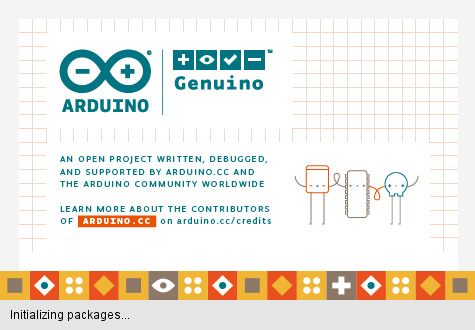
\includegraphics[width=0.4\textwidth]{figures/aride11.png}}
\caption{Arduino IDE.}
\label{aide}
\end{figure}

Menurut F. Djuandi dalam bukunya yang berjudul "Pengenalan Arduino" \cite{djuandi2011pengenalan} IDE merupakan singkatan dari Integrated Development Environment atau lingkungan terintegrasi yang digunakan untuk melakukan pengembangan. Dikatakan sebagai lingkungan karena melalui software inilah dilakukan pemrograman Arduino untuk melakukan fungsi - fungsi yang ditanamkan melalui sintaks pemrograman.Tampilan IDE ini bisa dilihat pada gambar \ref{aide}. IDE ini disediakan gratis dan bisa didapatkan secara langsung pada halaman resmi arduino yang bersifat open source. IDE ini juga sudah mendukung berbagai sistem operasi populer saat ini seperti Windows, Mac, dan Linux. Arduino menggunakan bahasa pemrograman sendiri yang menyerupai bahasa C. Pada bahasa pemrograman Arduino (Sketch) telah dilakukan beberapa perubahan untuk memudahkan para pemula dalam melakukan pemrograman dari bahasa aslinya. Sebelum dijual ke pasaran, IC microcontroller Arduino telah ditanamkan suatu program bernama Bootlader yang berfungsi sebagai penengah antara compiler Arduino dengan microcontroller.



\section{Proses Instalasi}

\begin{enumerate}
\item Pertama unduh terlebih dahulu installer IDE Arduino di https://www.arduino.cc/en/Main/Software. Pada halaman tersebut ada tiga macam installer yang dapat diunduh sesuai dengan Operating System yang kita pakai.
\break\\
\centerline{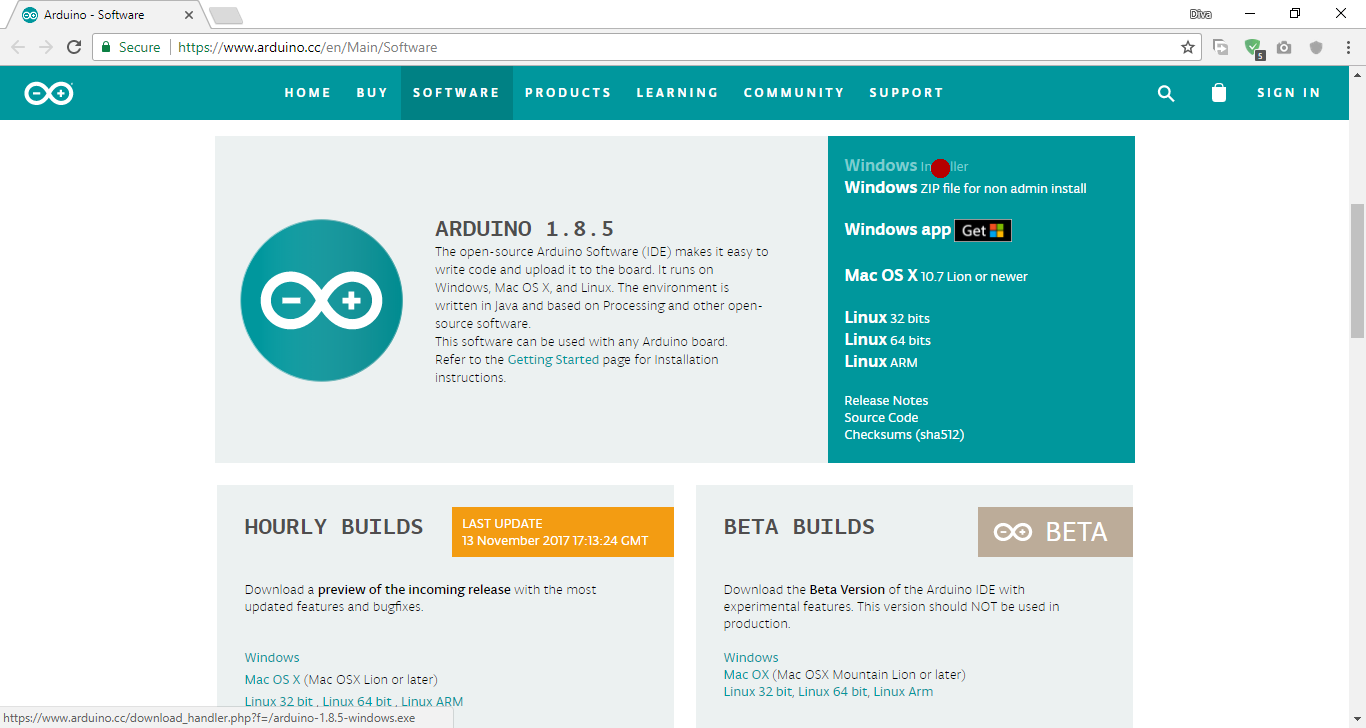
\includegraphics[width=0.9\textwidth]{figures/aride8.png}}
\item Kemudian pada halaman tersebut ada dua pilihan apakah kita ingin berkontribusi dengan memberikan uang sesuai dengan nominal yang tertera atau hanya mengunduh saja. Disini kita klik `Just Download' dan proses mengunduh dimulai.
\break\\
\centerline{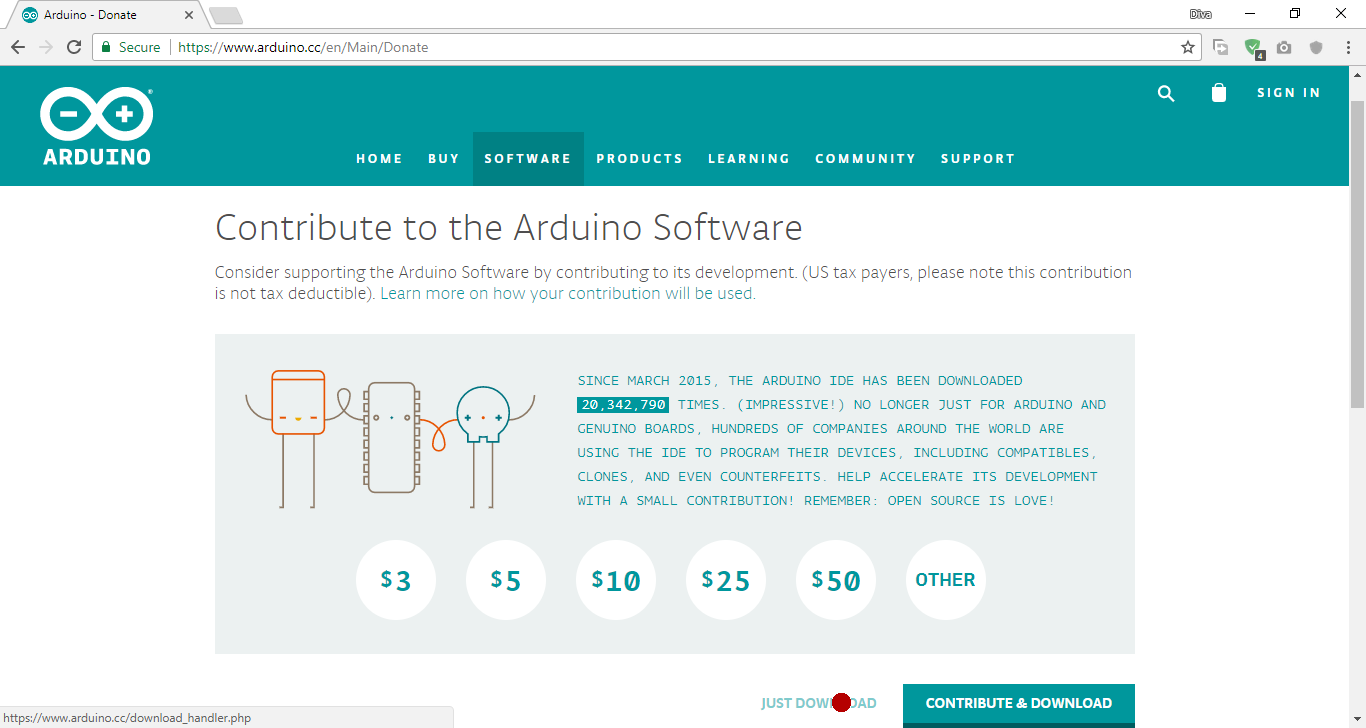
\includegraphics[width=0.9\textwidth]{figures/aride9.png}}
\item Setelah file installer telah selesai di unduh, lalu jalankan installer tersebut. Selanjutnya akan muncul jendela `Arduino Setup: License Agreement'. Lalu klik tombol `I Agree'.
\break\\
\centerline{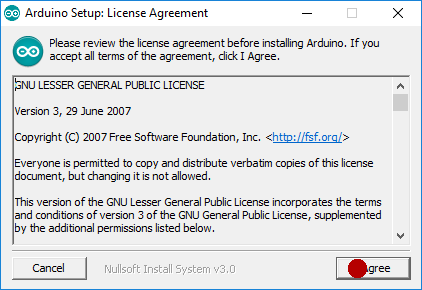
\includegraphics[width=0.9\textwidth]{figures/aride1.png}}
\item Selanjutnya akan muncul jendela `Arduino Setup: Installation Options'. Centang semua opsi yang ada, lalu klik `Next'.
\break\\
\centerline{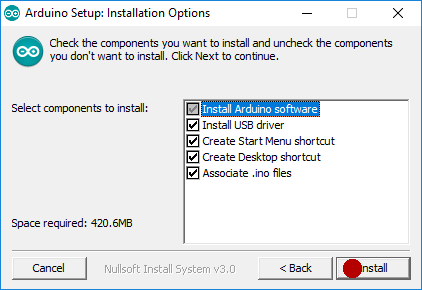
\includegraphics[width=0.9\textwidth]{figures/aride2.png}}
\item Setelah itu, akan muncul jendela `Arduino Setup: Installation Folder'. Kita diminta memilih folder instalasi Arduino.
\break\\
\centerline{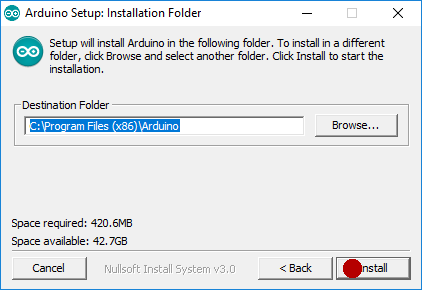
\includegraphics[width=0.9\textwidth]{figures/aride3.png}}
\item Selanjutnya proses instalasi akan dimulai.
\break\\
\centerline{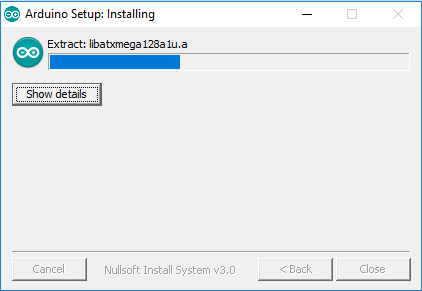
\includegraphics[width=0.9\textwidth]{figures/aride4.png}}
\item Pada saat melakukan proses instalasi, akan muncul jendela `Windows Security'. Jendela tersebut muncul apabila komputer kita belum terinstal driver - driver yang diperlukan. Klik tombol `Install'.
\break\\
\centerline{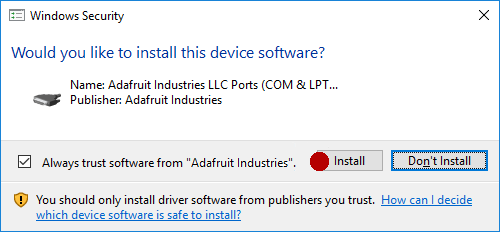
\includegraphics[width=0.9\textwidth]{figures/aride5.png}}
\break\\
\centerline{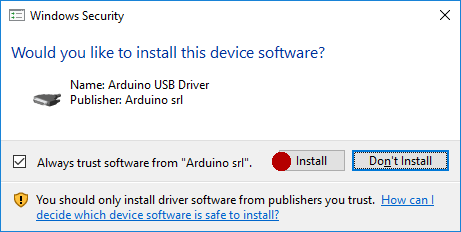
\includegraphics[width=0.9\textwidth]{figures/aride6.png}}
\break\\
\centerline{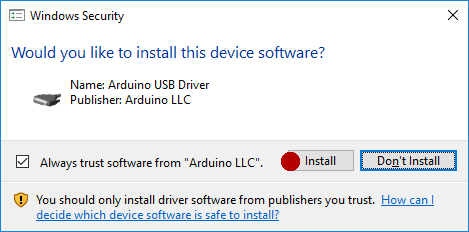
\includegraphics[width=0.9\textwidth]{figures/aride7.png}}
\item Selanjutnnya akan muncul jendela `Arduino Setup: Completed'. Jendela ini menandakan proses instalasi telah selesai. Klik tombol `Close'.
\break\\
\centerline{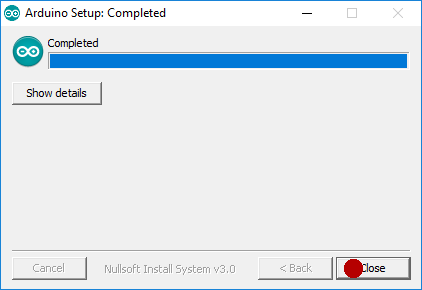
\includegraphics[width=0.9\textwidth]{figures/aride10.png}}
\item Setelah software IDE Arduino sudah terinstal. Coba cek di Start Menu Windows atau di desktop Anda, lalu jalankan aplikasi tersebut. Kemudian akan muncul splash screen seperti gambar di bawah ini.
\break\\
\centerline{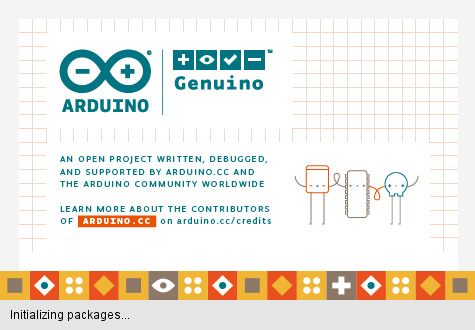
\includegraphics[width=0.9\textwidth]{figures/aride11.png}}
\item Selanjutnya akan muncul jendela IDE Arduino. Selamat Anda telah berhasil menginstal software IDE Arduino.
\break\\
\centerline{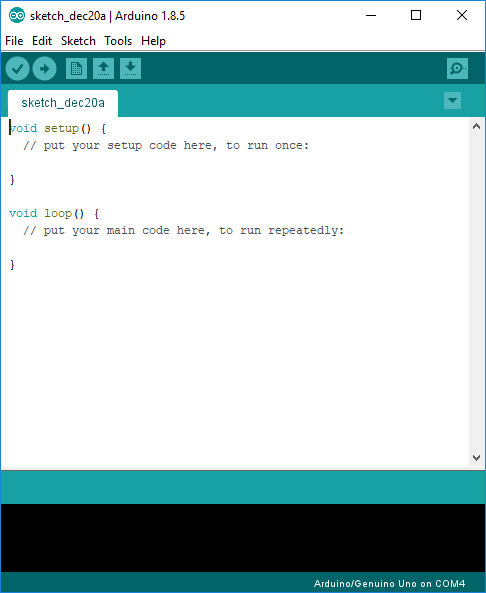
\includegraphics[width=0.9\textwidth]{figures/aride12.png}}
\end{enumerate}

\section{Fitur-Fitur IDE Arduino}

Arduino IDE dibuat dengan menggunakan bahasa pemrograman Java serta dilengkapi library C/C++. Arduino IDE merupakan hasil pengembangan dari software Processing yang kemudian diubah menjadi Arduino IDE khusus pemrograman dengan Arduino. IDE Arduino terdiri dari:

\begin{itemize}

\item Editor merupakan jendela yang digunakan oleh pengguna untuk mengubah dan menulis suatu program atau kode – kode dalam bahasa Processing.
\item Compiler merupakan sebuah modul untuk mengubah kode-kode program menjadi kode biner dikarenakan sebuah microcontroller tidak dapat memahami bahasa pemrograman dan yang hanya bisa memahami kode biner Saja. Oleh karena itu, compiler diperlukan dalam pemrograman.
\item Uploader merupakan sebuah modul yang berisi kode - kode biner atau sketch dari komputer ke dalam memory yang ada di dalam papan Arduino.
\end{itemize}

Program yang dibuat dengan menggunakan IDE Arduino disebut sebagai sketch. Sebuah sketch dibuat dalam suatu editor teks dan disimpan dengan ekstensi .ino. Teks editor pada Arduino Software memiliki beberapa fitur seperti cutting atau paste dan seraching atau replacing sehingga memudahkan kita dalam menulis kode program.

Pada Arduino IDE juga, terdapat semacam kotak pesan berwarna hitam yang berfungsi untuk menampilkan status program, seperti proses kompilasi, unggah program, dan pesan error. Pada bagian bawah paling kanan Arduino IDE, terdapat board yang terkonfigurasi beserta COM Ports yang digunakan.

\subsection{Verify}
Verify berfungsi untuk melakukan memeriksa kode - kode program yang telah kita buat apakah sudah sesuai dengan kaidah pemrograman yang ada atau belum.
\subsection{Upload}
Upload berfungsi untuk melakukan kompilasi kode - kode atau program yang telah kita buat sebelumnya menjadi kode biner agar dapat dipahami Arduino.
\subsection{New}
New berfungsi untuk membuat Sketch baru.
\subsection{Open}
Open berfungsi untuk membuka kembali sketch yang telah dibuat sebelumnya untuk dilakukan perubahan atau hanya diupload ulang ke Arduino.
\subsection{Save}
Save berfungsi untuk menyimpan Sketch yang telah kita buat.
\subsection{Serial Monitor}
Serial Monitor berfungsi untuk menampilkan data yang dipertukarkan atau dikirimkan antara sketch dengan arduino yang terhubung dengan port serialnya. Serial Monitor ini sangat berguna apabila kita ingin melakukan debugging atau yang dipertukarkan atau dikirimkan antara sketch dengan arduino pada port serialnya. Serial Monitor ini sangat berguna apabila kita ingin melakukan debugging atau membuat suatu program tanpa menggunakan LCD pada Arduino sebagai penampil nilai. Serial monitor ini dapat digunakan untuk menampilkan nilai dari proses dan pembacaan, serta pesan error.
\subsection{File}
Di dalam tab File berisi.
\begin{itemize}
\item New berfungsi untuk membuat sketch baru dengan bare minimum yang terdiri void setup() dan void loop(). 
\item Open berfungsi untuk membuka sketch yang pernah dibuat di dalam drive.
\item Open Recent berfungsi untuk mempersingkat waktu pembukaan file atau sketch yang baru-baru ini telah dibuat.
\item Sketchbook berfungsi untuk menunjukan hirarki sketch yang kita buat termasuk struktur foldernya.
\item Example berisi contoh – contoh dari pemrograman yang telah disediakan oleh pengembang Arduino, sehingga kita dapat mempelajari program-program dari contoh yang diberikan.
\item Close berfungsi untuk menghentikan dan menutup jendela Arduino IDE.
\item Save berfungsi untuk menyimpan sketch yang diubah atau baru dibuat.
\item Save as berfungsi untuk menyimpan sketch yang sedang dikerjakan atau sketch yang sudah disimpan dengan nama yang berbeda.
\item Page Setup berfungsi untuk mengatur tampilan page pada proses pencetakan.
\item Print berfungsi untuk mengirimkan file sketch ke mesin cetak untuk dicetak.
\item Preferences disini kita dapat merubah tampilan interface IDE Arduino.
\item Quit berfungsi untuk menutup semua jendela Arduino IDE.
\end{itemize}

\subsection{Edit}
Di dalam tab Edit berisi.
\begin{itemize}
\item Undo atau Redo berfungsi untuk mengembalikan perubahan yang telah dilakukan pada Sketch beberapa langkah mundur dengan Undo dan beberapa langkah maju dengan Redo.
\item Cut berfungsi untuk meremove teks yang terpilih pada editor dan menempatkan teks tersebut pada clipboard.
\item Copy berfungsi untuk menduplikasi teks yang terpilih ke dalam editor dan menempatkan teks tersebut pada clipboard.



%%%%%%%%%%%%%%%%%%%%%%%%%%%%%%%%%%%%%%%%%%%%%%%%%%%%%%%%%%%



\item Copy for Forum berfungsi untuk melakukan copy kode dari editor dan melakukan formating agar sesuai untuk ditampilkan dalam forum, sehingga kode tersebut bisa digunakan sebagai bahan diskusi dalam forum.
\item Paste berfungsi untuk menyalin data - data yang terdapat dalam clipboard, kedalam editor.
\item Select All berfungsi untuk melakukan pemilihan kode atau teks dalam halaman editor.
\item Comment atau Uncomment berfungsi untukmemberikan atau menghilangkan tanda // pada kode atau teks, dimana tanda tersebut menjadikan suatu baris kode sebagai komen dan tidak disertakan pada tahap kompilasi.
\item Increase atau Decrease Indent berfungsi untuk mengurangi atau menambahkan indentasi pada baris kode tertentu. Indentasi adalah “tab”.
\item Find berfungsi untuk memanggil jendela window find and replace, dimana kita bisa menggunakannya untuk menemukan variabel atau kata tertentu dalam program atau menemukan serta menggantikan kata tersebut dengan kata lain.
\item Find Next berfungsi untuk mencari kata setelahnya dari hasil kata pertama yang ditemukan.
\item Find Previous berfungsi untuk mencari kata sebelumnya dari hasil kata pertama yang ditemukan.
\end{itemize} 

\subsection{Sketch}
Di dalam tab Sketch berisi.
\begin{itemize}
\item Verify/Compile berfungsi untuk mengecek apakah sketch yang kamu buat ada kekeliruan dari segi sintaks atau tidak. Jika tidak ada kesalahan, maka sintaks yang kamu buat akan dikompile kedalam bahasa mesin.
\item Upload berfungsi mengirimkan program yang sudah dikompilasi ke Arduino Board.
\item Upload Using Programmer menu ini berfungsi untuk menuliskan bootloader kedalam IC Mikrokontroler Arduino. Pada kasus ini kamu membutuhkan perangkat tambahan seperti USBAsp untuk menjembatani penulisan program bootloader ke IC Mikrokontroler.
\item Export Compiled Binary memiliki fungsi untuk menyimpan file dengan ekstensi .hex, dimana file tersebut dapat disimpan sebagai arsip untuk diupload ke board lain menggunakan tools yang berbeda.
\item Show Sketch Folder, berfungsi membuka folder sketch yang saat ini dikerjakan.
\item Include Library, berfunsi menambahkan library/pustaka kedalam sketch yang dibuat dengan menyertakan sintaks \#include di awal kode. Selain itu kita juga dapat menambahkan library eksternal dari file .zip kedalam Arduino IDE.
\item Add File…, berfungsi untuk menambahkan file kedalam sketch arduino (file akan dikopikan dari drive asal). 
File akan muncul sebagai tab baru dalam jendela sketch.
\end{itemize}
\subsection{Tools}
Di dalam tab Tools berisi.
\begin{itemize}
\item Auto Format berfungsi melakukan pengatran format kode pada jendela editor
\item Archive Sketch berfungsi menyimpan sketch kedalam file .zip
\item Fix Encoding \& Reload berfungsi memperbaiki kemungkinan perbedaan antara pengkodean peta karakter editor dan peta karakter sistem operasi yang lain.
\item Serial Monitor berfungsi menampilkan jendela serial monitor agar dapat melihat proses pertukaran data.
\item Board berfungsi mengkonfigurasi dan memilih board yang kita gunakan.
\item Port memilih port sebagai kanal komunikasi antara software dengan hardware.
\item Programmer menu ini digunakan ketika kamu hendak melakukan pemrograman chip mikrokontroller tanpa menggunakan koneksi Onboard USB-Serial. Biasanya digunakan pada proses burning bootloader.
\item Burn Bootloader berfungsi mengizinkan kita mengcopykan program bootloader ke dalam IC mikrokontroler.
\end{itemize}

\subsection{Help}
Menu help berisikan file-file dokumentasi yang berkaitan dengan masalah yang sering muncul, serta penyelesaiannya. Selain dokumentasi yang telah disediakan kita juga diberikan link untuk menuju Arduino Forum. Forum tersebut membahas berbagai masalah yang ditemukan mengenai Arduino.

\subsection{Sketchbook}
Arduino Software IDE menggunakan konsep sketchbook. Sketchbook merupakan standar penyimpanan dan peletakan file program. Sketch yang telah kita buat dapat dibuka dari File - Sketchbook, atau dengan menu Open.

\subsection{Tabs, Multiple Files, dan Compilations}
Mekanisme ini mengizinkan kita dalam melakukan manajemen sketch, dimana lebih dari satu file dibuka dalam tab yang berbeda.

\subsection{Uploading}
Mekanisme untuk mengcopykan file hasil kompilasi program ke dalam IC mikrokontroler Arduino. Sebelum melakukan uploading, yang perlu kita pastikan sebelumnya adalah jenis board yang kita gunakan dan COM Ports dimana keduanya terletak pada menu Tools - Board dan Tools - Port.

\subsection{Library}
Library merupakan file yang memberikan fungsi ekstra dari sketch yang kita buat. Untuk menginstal Library pihak ketiga alias Library bukan dari Arduino, maka dapat dilakukan dengan Library Manager, Import file .zip, atau copy paste secara manual di folder libraries pada Documents di platform Windows.

\subsection{Serial Monitor}

Serial monitor merupakan sebuah jendela yang digunakan untuk menunjukan data yang dipertukarkan antara komputer dan arduino selama beroperasi. Dengan adanya serial monitor ini kita dapat melihat nilai hasil operasi atau pesan debugging. Selain melihat data, kita juga bisa mengirimkan data ke Arduino melalui serial monitor ini, caranya dengan memasukkan data pada text box dan menekan tombol send untuk mengirimkan data. Hal penting yang harus kita perhatikan adalah menyamakan baudrate antara serial monitor dengan Arduino board. Untuk menggunakan kemampuan komunikasi serial ini, pada Arduino, di bagian fungsi void setup(), diawali dengan instruksi Serial.begin diikuti dengan nilai baudrate.


\subsection{Preferences}
Preferences digunakan untuk mengatur beberapa hal dalam penggunaan Arduino Software IDE, seperti lokasi dimana penyimpanan sketchbook, bahasa yang digunakan pada Arduino Software IDE, ukuran font, dan lain sebagainya. Kita dapat mengatur preferences pada menu file yang dapat dijumpai pada platform Windows dan Linux.

\subsection{Language Support}
Language Support merupakan pilihan bahasa yang dapat disesuaikan pada Software Arduino IDE. Language Support dapat ditemukan dengan menekan Ctrl + Comma atau pada menu file - preferences.

\subsection{Boards}
Pemilihan board pada Arduino Software IDE, berdampak pada dua parameter yaitu kecepatan CPU dan baudrate yang digunakan ketika melakukan kompilasi dan meng-upload sketch. Beberapa contoh board yang dapat digunakan dengan Arduino Software IDE dapat dilihat pada tabel \ref{table:boardarduino}.

%%%%%%%%%%%%%%%%%%%%%%%%%%%%%%%%%%%%%%%%%%%%%%%%%%%%%%%%%%%

\begin{table}[!ht]
\centering
\begin{tabular}{ |l|l| }
\hline
Arduino/ Genuino Uno & Menggunakan ATmega328 dan berjalan pada \\
& clock 16 MHz dengan auto-reset, memiliki 6 Input \\
\hline
Arduino Nano w/ ATmega328 & Menggunakan ATmega328 dan berjalan pada \\
& clock 16 MHz dengan auto-reset. memiliki 6 Input Analog.\\
\hline
Arduino/ Genuino Mega 2560 & Menggunakan ATmega2560 dan berjalan pada \\
& clock 16 MHz dengan auto-reset, memiliki 16 Input \\
& Analog, 54 Digital I/O dan 15 PWM. \\
\hline
Arduino Mega & Menggunakan ATmega1280 dan berjalan pada \\
& clock 16 MHz dengan auto-reset, memiliki 16 Input \\
& Analog, 54 Digital I/O dan 15 PWM.\\
\hline
Arduino Mega ADK & Menggunakan ATmega2560 dan berjalan pada \\
& clock 16 MHz dengan auto-reset, memiliki 16 Input \\
& Analog, 54 Digital I/O dan 15 PWM. \\
\hline
Arduino Leonardo & Menggunakan ATmega32u4 dan berjalan pada \\
& clock 16 MHz dengan auto-reset, memiliki 12 Input \\
& Analog, 20 Digital I/O dan 7 PWM.\\
\hline
Arduino Micro & Menggunakan ATmega32u4 dan berjalan pada \\
& clock 16 MHz dengan auto-reset, memiliki 12 Input \\
& Analog, 20 Digital I/O dan 7 PWM. \\
\hline
Arduino Esplora & Menggunakan ATmega32u4 dan berjalan pada \\
& clock 16 MHz dengan auto-reset.\\
\hline
Arduino Mini w/ ATmega328 & Menggunakan ATmega328 dan berjalan pada \\
& clock 16 MHz dengan auto-reset, memiliki 8 Input \\
& Analog, 14 Digital I/O dan 6 PWM.\\
\hline
Arduino Ethernet & Equivalent to Arduino UNO with an Ethernet shield: \\
& An ATmega328 dan berjalan pada clock 16 MHz \\ 
& dengan auto-reset, memiliki 6 Input Analog, 14 Digital \\
& I/O dan 6 PWM.\\
\hline
Arduino Fio & Menggunakan ATmega328 dan berjalan pada \\
& clock 8 MHz dengan auto-reset. Memiliki kesamaan \\ 
& dengan Arduino Pro atau Pro Mini (3.3V, 8 MHz) \\ 
& w/ ATmega328, memiliki 6 Input Analog, 14 Digital I/O \\ 
& dan 6 PWM.\\
\hline
Arduino BT w/ ATmega328 & Menggunakan ATmega328 dan berjalan \\
& pada clock 16 MHz. Bootloader dengan ukuran (4 KB) \\
& termasuk kode untuk melakukan inisialisasi pada modul \\
& bluetooth, memiliki 6 Input Analog, 14 Digital I/O and 6 PWM.\\
\hline
LilyPad Arduino USB & Menggunakan ATmega32u4dan berjalan \\
& pada clock 8 MHz dengan auto-reset, memiliki 4 Input \\
& Analog, 9 Digital I/O dan 4 PWM. \\
\hline
LilyPad Arduino & Menggunakan ATmega168 atau ATmega132 \\
& dan berjalan pada clock 8 MHz dengan auto-reset, \\
&memiliki 6 Input Analog, 14 Digital I/O dan 6 PWM. \\
\hline
Arduino Pro or Pro Mini & Menggunakan ATmega328 dan berjalan pada \\
(5V, 16 MHz) w/ ATmega328 & clock 16 MHz dengan auto-reset. Memiliki \\
 & kesamaan dengan Arduino Duemilanove atau \\
 & Nano w/ ATmega328,memiliki 6 Input Analog,\\
 & 14 Digital I/O dan 6 PWM. \\
\hline
Arduino NG or older w/ ATmega168 & Menggunakan ATmega168 dan berjalan \\
& pada clock 16 MHz without auto-reset. \\
& Proses kompilasi dan upload sama dengan \\
& Arduino Diecimila atau Duemilanove \\
& w/ ATmega168,memiliki 16 Input Analog,\\
& 14 Digital I/O and 6 PWM. \\
\hline
Arduino Robot Control & Menggunakan ATmega328 dan berjalan pada\\
& clock 16 MHz dengan auto-reset. \\
\hline
Arduino Robot Motor & Menggunakan ATmega328 dan berjalan pada \\
& clock 16 MHz dengan auto-reset. \\
\hline
Arduino Gemma & Menggunakan ATtiny85 dan berjalan pada \\
& clock 8 MHz dengan auto-reset, 1 Analog In,\\
& 3 Digital I/O and 2 PWM. \\
\hline
\end{tabular}
\caption{Board Arduino.}
\label{table:boardarduino}
\end{table}